%!TEX root = ../ArticleCalib_main.tex


%%%%%%%%%%%%% FIGURE 10  Calibration experimentale laser & Corrélations

\begin{figure}[htbp]
\begin{center}
\captionsetup[subfigure]{position=top, labelfont=bf, textfont=normalfont, singlelinecheck=off, justification=raggedright }

\subfloat[]{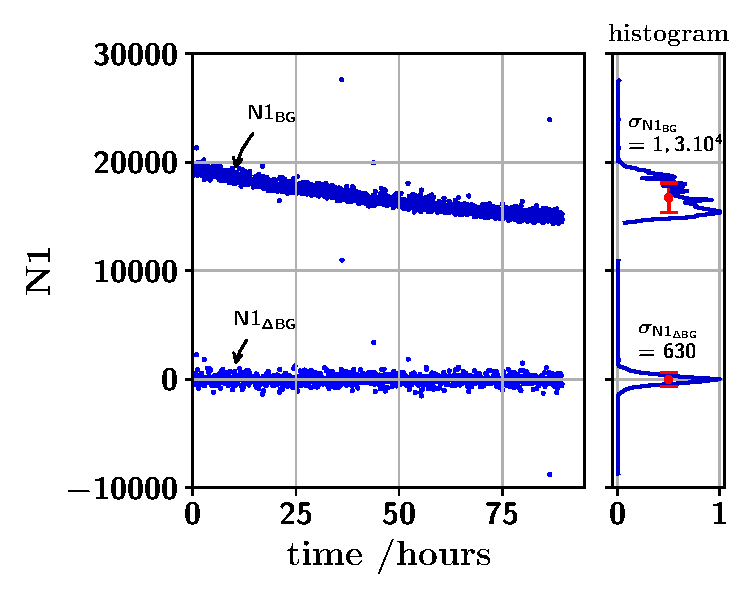
\includegraphics[width=0.4\linewidth]{fig10_CalibExp_Correlation/fig10A_BGBG_CorrelationsProches_fluctuations.pdf}\label{fig:CalibCorrel:A}} \qquad
\subfloat[]{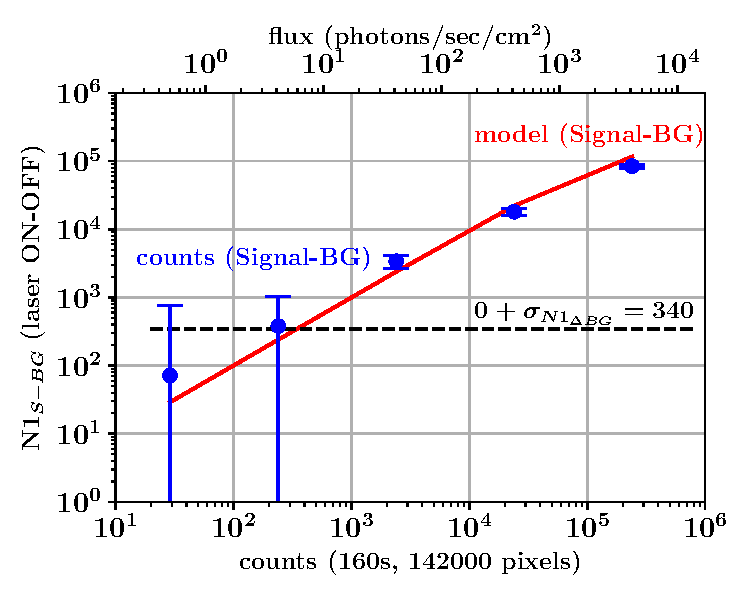
\includegraphics[width=0.4\linewidth]{fig10_CalibExp_Correlation/fig10B_CalibLaser.pdf}\label{fig:CalibCorrel:B}} 

\subfloat[]{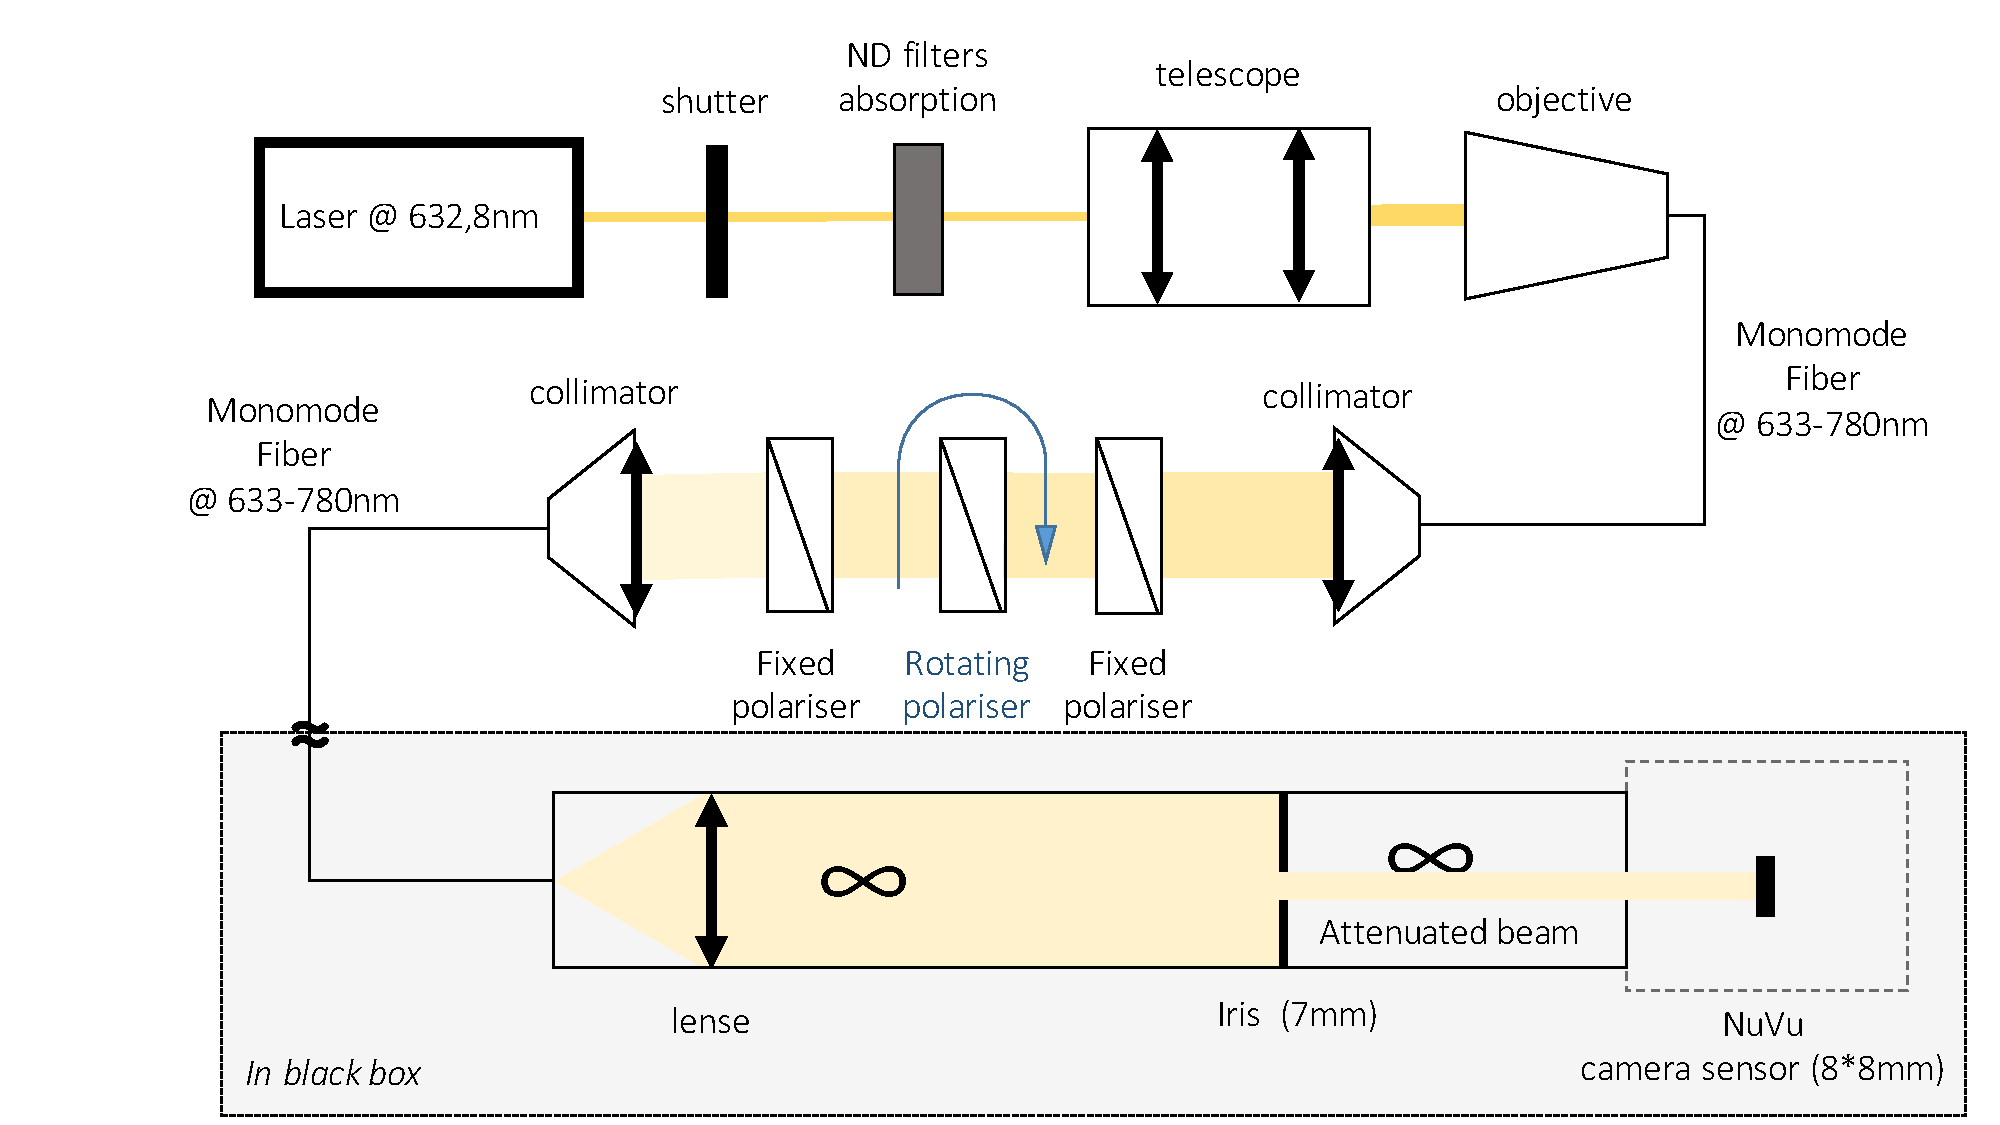
\includegraphics[width=0.7\linewidth]{fig10_CalibExp_Correlation/fig10C_CalibLaser.pdf}\label{fig:CalibCorrel:C}} \\



\caption{
{\bf Experimental calibration and noise subtraction to free measurement from low frequencies noise variations}. 
\subref{fig:CalibCorrel:A} : Raw data taken in the most possible darkness on the entire surface sensor, (ie shutter closed), (N1$_{BG}$) show a slow relaxation process. 
When subtracting neighbouring data points (N1$_{\Delta BG}$),  the observed variance is lower than the expected variance for non correlated measurements, and only high frequency fluctuation from the camera sensor noise remains (variation between two neighbouring points).
The distribution of both set of data point is respectively shown by the histograms.
\subref{fig:CalibCorrel:B} : Calibrated flux detection with the NuVu camera and comparaison of the experimental results and the model describing the behavior of the NuVu camera.
The datas are the average of the difference between the average photons counts inside the area illuminated by the laser  beam (40 mm²  diameter disk) during the  time of exposure of optimal density  (160sec), and  the environmental noise (determined with the shutter open while the LASER is off). 
All statistics are made on the difference between the signal (camera shutter open) and the camera noise (camera shutter closed : BG).
The limit of detection (black dotted line) represents the noise floor, and corresponds to $5.8 counts /\mathrm{cm}^{-2}s$.
\subref{fig:CalibCorrel:C}  : Experimental setup to produce a beam of calibrated low light fluxes. The final optical elements are placed in a thorlab SM1 tube and fixed on the camera via c-mount. 
We only select the central zone of the infinite attenuated beam to have a better average flux uniformity throughout the beam section.
}
\label{fig:CalibCorrel}
\end{center}
\end{figure}
